\documentclass[12pt,a4paper]{article}

% Улучшенный поиск русских слов в полученном pdf-файле
% добавлять до пакета fontenc
\usepackage{cmap}

\usepackage[T2A]{fontenc}
\usepackage[utf8]{inputenc}
\usepackage[russian]{babel}
\usepackage{graphicx}
\usepackage{amsmath,amssymb}

% Управление цветами различных элементов. Например - гиперссылок
\usepackage{color}

% Пакет, добавляющий работающие ссылки на разделы, формулы, литературы
% и прочие рисунки и таблицы
\usepackage{hyperref}

%\usepackage[total={17cm, 23cm}, top=2.5cm, left=1.5cm]{geometry}
\usepackage[top=2.5cm, left=1.5cm]{geometry}

\graphicspath{{images/}}

\title{\bf Исследование неравновесной критической динамики трехмерной сильнонеупорядоченной модели Изинга}
\author{\it Автор~А.~А., Автор~А.~Б., Автор~А.~В., Автор~А.~Г.}
\date{\textit{\small Омский государственный университет им. Ф.М.~Достоевского \\644077, Омск, Россия}}

\pagestyle{headings}

\hyphenation{кон-центра-ция} % просто для примера, не хотим разделить центральные два слога

% Убрать цветные рамки от всех внутренних ссылок документа.
% Команда definecolor - предоставляется пакетом color
\definecolor{linkcolor}{rgb}{0,0,0}
\definecolor{citecolor}{rgb}{0,0,0}
\hypersetup{colorlinks, linkcolor={linkcolor}, citecolor={citecolor}}
%%%%%%%%%

\begin{document}

\maketitle
\thispagestyle{headings} % Для применения требуемого стиля к заглавной странице

\begin{abstract}
Осуществлено численное исследование критического поведения изинговских магнетиков в условиях сильного разбавления методом коротко-временной динамики. Определены динамические и статические характеристики критического поведения сильнонеупорядоченной трехмерной модели Изинга с  учетом поправок к скейлингу. Показано наличие нового класса универсальности для сильнонеупорядоченных систем.
\end{abstract}


\section{Введение}

Влиянию дефектов на критическую эволюцию модели Изинга посвящено значительное число работ. Это объясняется тем, что согласно критерию Харриса \cite{lit:Harris}, примеси влияют на критическое поведение системы только в том случае, если критический индекс теплоемкости бездефектной системы $\alpha > 0$. В этом случае проявляется новый класс универсальности с показателями, отличными от чистой системы. В случае теоретического описания ферромагнетиков, только модель Изинга удовлетворяет этому критерию. В классификации Вейнриба-Гальперина \cite{lit:HalperinHoenberg} подобные системы соответствует модели A.

Исследования методами ренормализационной группы (РГ) и методами Монте\cdash--~{}Карло (МК) показали, что при малой концентрации дефектов $(1-p) \ll 1$, где $p$ - концентрация спинов, реализуется новое критическое поведение \cite{lit:Folk}. В тоже время актуальным остается вопрос о влиянии сильного разбавления системы немагнитрыми примесями. Из теории перколяции известно, что при некоторой концентрации спинов $p^{(s)}_{c}$, называемом порогом спиновой перколяции, спины на двухмерной или трехмерной решетке могут образовывать протекающие структуры с возникновением спонтанной намагниченности при $T < T_c(p)$ и $p > p^{(s)}_{c}$. Такое же поведение можно ожидать и для дефектов структуры при превышении порога перколяции примесей $p^{(imp)}_{c}$. Для трехмерной кубической решетки, в терминах концентрации спинов, порог перколяции дефектов $p^{(imp)}_{c} = 1 - p^{(s)}_{c} \approx 0.69$. Системы с концентрацией спинов $p^{(imp)}_{c} < p < 1$ можно называть слабо неупорядоченными, с $p_{c}^{s} < p < p_{c}^{(imp)}$ -- сильно неупорядоченными.

Большинство численных исследований проводятся методом коротко\cdash--~{}временной динамики (МКД). Этот метод основан на существовании универсальных временных зависимостей для термодинамических характеристик на раннем этапе эволюции, когда системы еще не достигла состояния термодинамического равновесия. Первоначально в статье \cite{lit:Janssen} демонстрируется универсальное скейлинговое поведение для функции отклика $G(r,t,t')$ и параметра порядка -- намагниченность в случае ферромагнетика -- $m(t)$ для системы, находящейся в неравновесном начальном состоянии. Ранний этап динамической эволюции характеризуется показателями $\theta$ и $\theta'$ соответственно.
\begin{equation} \label{eq0}
 G(r,t,t') \sim (t/t')^{\theta},  m(t) \sim t^{\theta'}
\end{equation}
Одним из нетривиальных эффектов коротковременной динамики является возрастание намагниченности при эволюции системы из начального состояния с $m_0 \ll 1$. Необходимо подчеркнуть, что этот эффект происходит на временах порядка $t < t_cr \sim m_{0}^{-1/(\theta'+\beta/z\nu)}$. Возрастание намагниченности сменяется спаданием $m(t) \sim t^{-\beta/z\nu}$ для $t \gg t_{cr}$. В дальнейшем   исследования универсального поведения различных термодинамических функций на раннем этапе эволюции различных систем привели к возможности определения как статических критических индексов $\beta$, $\nu$, так и динамических критических показателей $z$ и $\theta'$ \cite{lit:Huse} -- \cite{lit:Luo}.

Предыдущие исследования Монте-Карло не дают однозначного ответа о зависимости или независимости критических показателей от концентрации дефектов. Так, в работе \cite{lit:Schehr} произведен расчет индекса $\theta'$ для диапазона концентраций $p = [0.49..0.8]$. Полученное значение $\theta' = 0.10(2)$  для всех $p$. Детали и обсуждение этого результата приведено ниже. В работе \cite{lit:Hasenbusch} декларируется существование универсального динамического критического индекса $z = 2.35(2)$ для всех $p$, что противоречит как экспериментальным данным \cite{lit:Rosov88}, так и теоретико-полевому описанию в двух- и трех-петлевом приближении $\varepsilon$-разложения \cite{lit:Prudnikov_FT}.

Данная работа посвящена исследованию критического поведения трехмерной сильнонеупорядоченной модели Изинга со спиновыми концентрациями $p = 0.5$ и $0.6$. В следующем разделе представлено описание методов и модели исследования. В разделе 3 приводится результаты для полученных критических характеристик. В разделе 4 сделан анализ полученных результатов и их сравнение с результатами дургих работ.

\section[3D модель Изинга]{Моделирование неупорядоченной трехмерной модели Изинга}

Гамильтониан трехмерной структурно неупорядоченной модели Изинга определяется выражением:
\begin{eqnarray} \label{ham}
H =-J\sum_{\langle i,j\rangle}p_i p_j S_i S_j,
\end{eqnarray}
где $J>0$ - константа обменного взаимодействия ближайших спинов $S_i$, $S_i$ - спин узла, принимающий значения $\pm 1$, $p_i$ - числа заполнения, характеризующие наличие $\delta$-коррелированного беспорядка в системе: $p_i = 1$, когда в узле $i$ находится спин, и $p_i = 0$, в случае немагнитного атома.

На основе  ренорм-группового анализа в работе Янссена \cite{lit:Janssen} показано, что для $k$-го момента намагниченности реализуется скейлинговая форма:
\begin{equation} \label{mk}
\begin{split}
m^{(k)} \left( t, \tau, L, m_0 \right) & =b^{- k\beta / \nu } \\
        & \times m^{(k)}\left( b^{-z} t, \ b^{1/\nu} \tau, \ b^{-1}L, \ b^{x_0}m_0 \right).
\end{split}
\end{equation}
В (\ref{mk}) $b$  - пространственный масштабный фактор, $\tau=(T-T_c)/T_c$ - приведенная температура, $\beta$ и $\nu$ - статические критические индексы, $z$ - динамический индекс, $x_0$ - новый независимый критический индекс, задающий масштабную размерность начального значения намагниченности $m_0$.

При моделировании различают два начальных состояния системы: $m_0 = 1$ и $m0 \ll 1$. Первое из них, соответствующее начаьному состоянию системы с $T = 0$, можно назвать низкотемпературным, второе - выкокотемпературным начальным состоянием.

На начальном этапе релаксации системы корреляционная длина еще достаточно мала и конечность размера моделируемой системы не оказывает существенного влияния. Рассматривая в (\ref{mk}) $m_0 = 1$ и полагая $b = t^{1/z}$, получаем намагниченность в виде:
\begin{equation} \label{mupr}
\begin{split}
M \left( t, \tau \right) & = b^{- \beta / \nu z } \times M\left( 1, t^{1/\nu z}\tau \right) \\
       & \sim t^{- \beta / \nu z} \left(1 + At^{1/\nu z}\tau + O(\tau^2) \right).
\end{split}
\end{equation}
В критической точке $\tau = 0 $ $M(t) \sim t^{- \beta / \nu z}$. Исследуя релаксационный процесс системы из начального низкотемпературного состояния, полезно определять временные зависимости для логарифмической производной $\partial_{\tau} ln M(t)$ и кумулянта $U_{2}(t)=\frac{M^{2}(t)}{(M(t))^2} - 1$:
\begin{equation} \label{utwo}
\begin{split}
\partial_{\tau} ln M(t) & \sim t^{1/\nu z}, \\
        U_{2}(t) & \sim t^{d/z}.
\end{split}
\end{equation}
Вместе с намагниченностью, анализ данных величин позволяет определить значения динамического $z$ и статических $\beta, \nu$ ритических индексов.

В случае $m_0 \ll 1$ намагниченность характеризуется следующей скейлинговой зависимостью:
\begin{equation} \label{mnonupr}
\begin{split}
M \left( t, \tau, m_0 \right)= m_{0}t^{\theta'} \left(1 + At^{1/\nu z}\tau + O(\tau^2, m_{0}^{2}) \right),
\end{split}
\end{equation}
где $\theta'$ - новый независимый критический индекс. В критической точке $\tau \to 0$
\begin{equation} \label{mtheta}
\begin{split}
M &\left( t \right) \sim t^{\theta'}
\end{split}
\end{equation}
Рассматривая второй момент намагниченности из (\ref{mk}), получаем следующую зависимость:
\begin{equation} \label{mtt}
\begin{split}
M^{(2)} \left( t \right) \sim t^{-2\beta / \nu}M^{(2)} \left( 1, t^{-1/z}L \right).
\end{split}
\end{equation}
Как указано выше, в начале кртической эволюции пространственная корреляционная длина достаточно мала, даже в $T_c$. В этом случае можно заключить, что\\ $M^{(2)} \left( 1, t^{-1/z}L \right) \sim L^{-d}$, где $d$ - размерность системы. Подставляя в (\ref{mtt}), получаем:
\begin{equation} \label{mtt_scail}
\begin{split}
M^{(2)} \left( t \right) \sim t^{c_2}, c_2 = \left( d - 2\beta / \nu \right)\frac{1}{z}.
\end{split}
\end{equation}
Другой интерисующей нас величиной является автокорреляционная функция $A(t)$. Ее скейлинговое соотношение имеет вид:
\begin{equation} \label{at_scail}
\begin{split}
  A\left( t \right) \sim t^{-c_a}, c_a = \left( \frac{d}{z} - \theta' \right).
\end{split}
\end{equation}
Для получения динамического индекса можно воспользоваться методом, ведённым в работе \cite{lit:Alves}. Авторы рассматривают временное поведение кумулянта:
\begin{equation} \label{ftt}
\begin{split}
F_{2} \left( t \right) = \frac{ M^{2} \left( t \right) |_{m_{0}=0} }{ \left( M \left( t \right) |_{m_{0}=1} \right)^{2} },
\end{split}
\end{equation}
где эволюция намагниченности исследуются для различных начальных состояний - низкотемпературного с $m_0 = 1$ и высокотемпературного с $m_0 \ll 1$. В критической точке данный кумулянт имеет следующую временную зависимость:
\begin{equation} \label{ft_scail}
\begin{split}
F_{2} \left( t \right) \sim \frac{ t^{ \left( d - 2\beta / \nu \right)\frac{1}{z} } }{ t^{-2\beta / \nu z} } \sim t^{d/z} .
\end{split}
\end{equation}
Вычисление кумулянта (\ref{ftt}) используется для непосредственного определения критического индекса $z$.

В данной работе вычсление критических характеристик проводилось на кубической решетке с линейным размером $L = 128$ для концентраций спинов $p = 0.5$ и $0.6$. Нами было проведено исследования двух начальных состояний системы - с $m_0 = 1$ и $m_0 \ll 1$.  Динамическая эволюция системы моделировалась посредством алгоритма Метрополиса. На решетке задавались периодические граничные условия. В процессе моделирования вычислялись намагниченность и автокорреляционная функция расчитывались по формулам:
\begin{equation} \label{m_calc}
m(t)=\left[ \left<  \frac{1}{pL^3} \sum_{i}^{pL^3} p_i {S_i}(t) \right>\right],
\end{equation}

\begin{equation} \label{A_calc}
A(t)=\left[ \left< \frac{1}{pL^3} \sum_{i}^{pL^3} p_i {S_i}(t){S_i}(0) \right>\right],
\end{equation}
где угловые скобки обозначают статистическое усреднение по реализациям требуемого начального состояния, а квадратные скобки - усреднение по различным примесным конфигурациям.

В качестве единицы времени использовался шаг Монте-Карло на спин - $MCs/s$ - означающий переворот всех спинов системы в единицу времени. Поведение систем исследовалось на временах до 3000 $MCs/s$. Для моделирования использовались критические температуры, определенные в работе \cite{lit:Tc}:
\begin{equation} \label{tc}
  \begin{split}
    p = 0.5, T_c = 1.84509(6)  \\
    p = 0.6, T_c = 2.42413(9)
  \end{split}
\end{equation}

Статистика исследования составляет порядка $10^4$ примесных конфигураций для каждой из моделируемых систем. При моделирвании  из начального состояния с $m_0 \ll 1$ каждая конфигурация дополнительно усреднялись по 25 прогонкам - для получения статистического усреднения по реализации требуемого начального состояния с малой намагниченностью. Для получения статистической погрешности, все данные разбивались на группы и вычислялись критические индексы. Затем по набору полученных показателей вычислялась статистическая погрешность. В данной работе все данные разбивались на 5 групп.

\section[Критические индексы]{Расчёт критических индексов трехмерной неупорядоченной модели Изинга}

\subsection{Динамика системы из начального неравновесного состояния с $m_0 = 1$}
В процессе моделирования осуществлялось вычисление намагниченности, ее логарифмической производной и кумулянта $U_2$ для вычисления критических индексов $\beta$, $\nu$ и $z$ в соотвествии с формулами (\ref{mupr}) - (\ref{utwo}). На рис.~\ref{fig:m1_all} приведены временные зависимости намагниченности для систем со спиновой концентрацией $p = 0.5$ и $p = 0.6$, полученные при моделировании системы с низкотемпаратурным начальным состоянием.

\begin{figure}[h]
\begin{center}

\begin{minipage}{6.77cm}
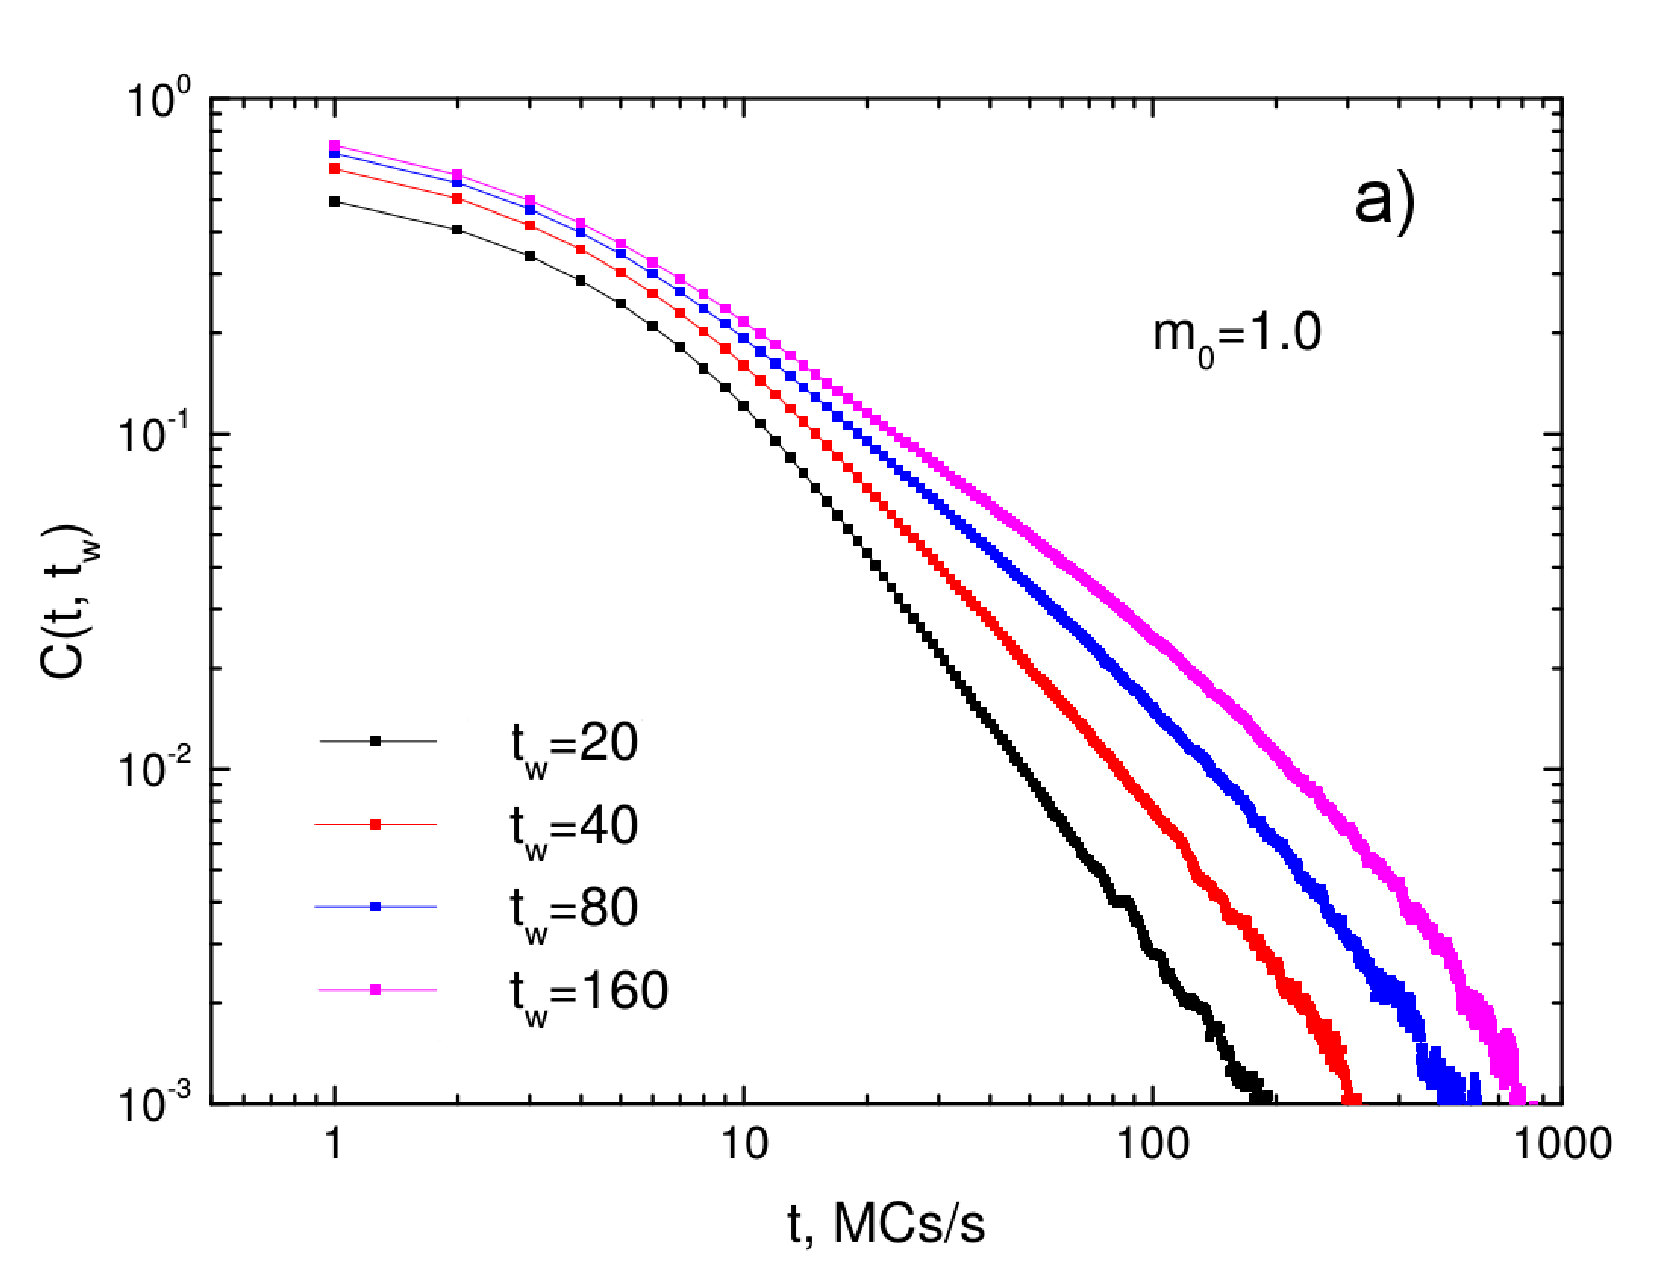
\includegraphics[width=6.77cm]{corr_ageing_1}
\end{minipage}\hspace{0.85cm}%
\begin{minipage}{6.77cm}
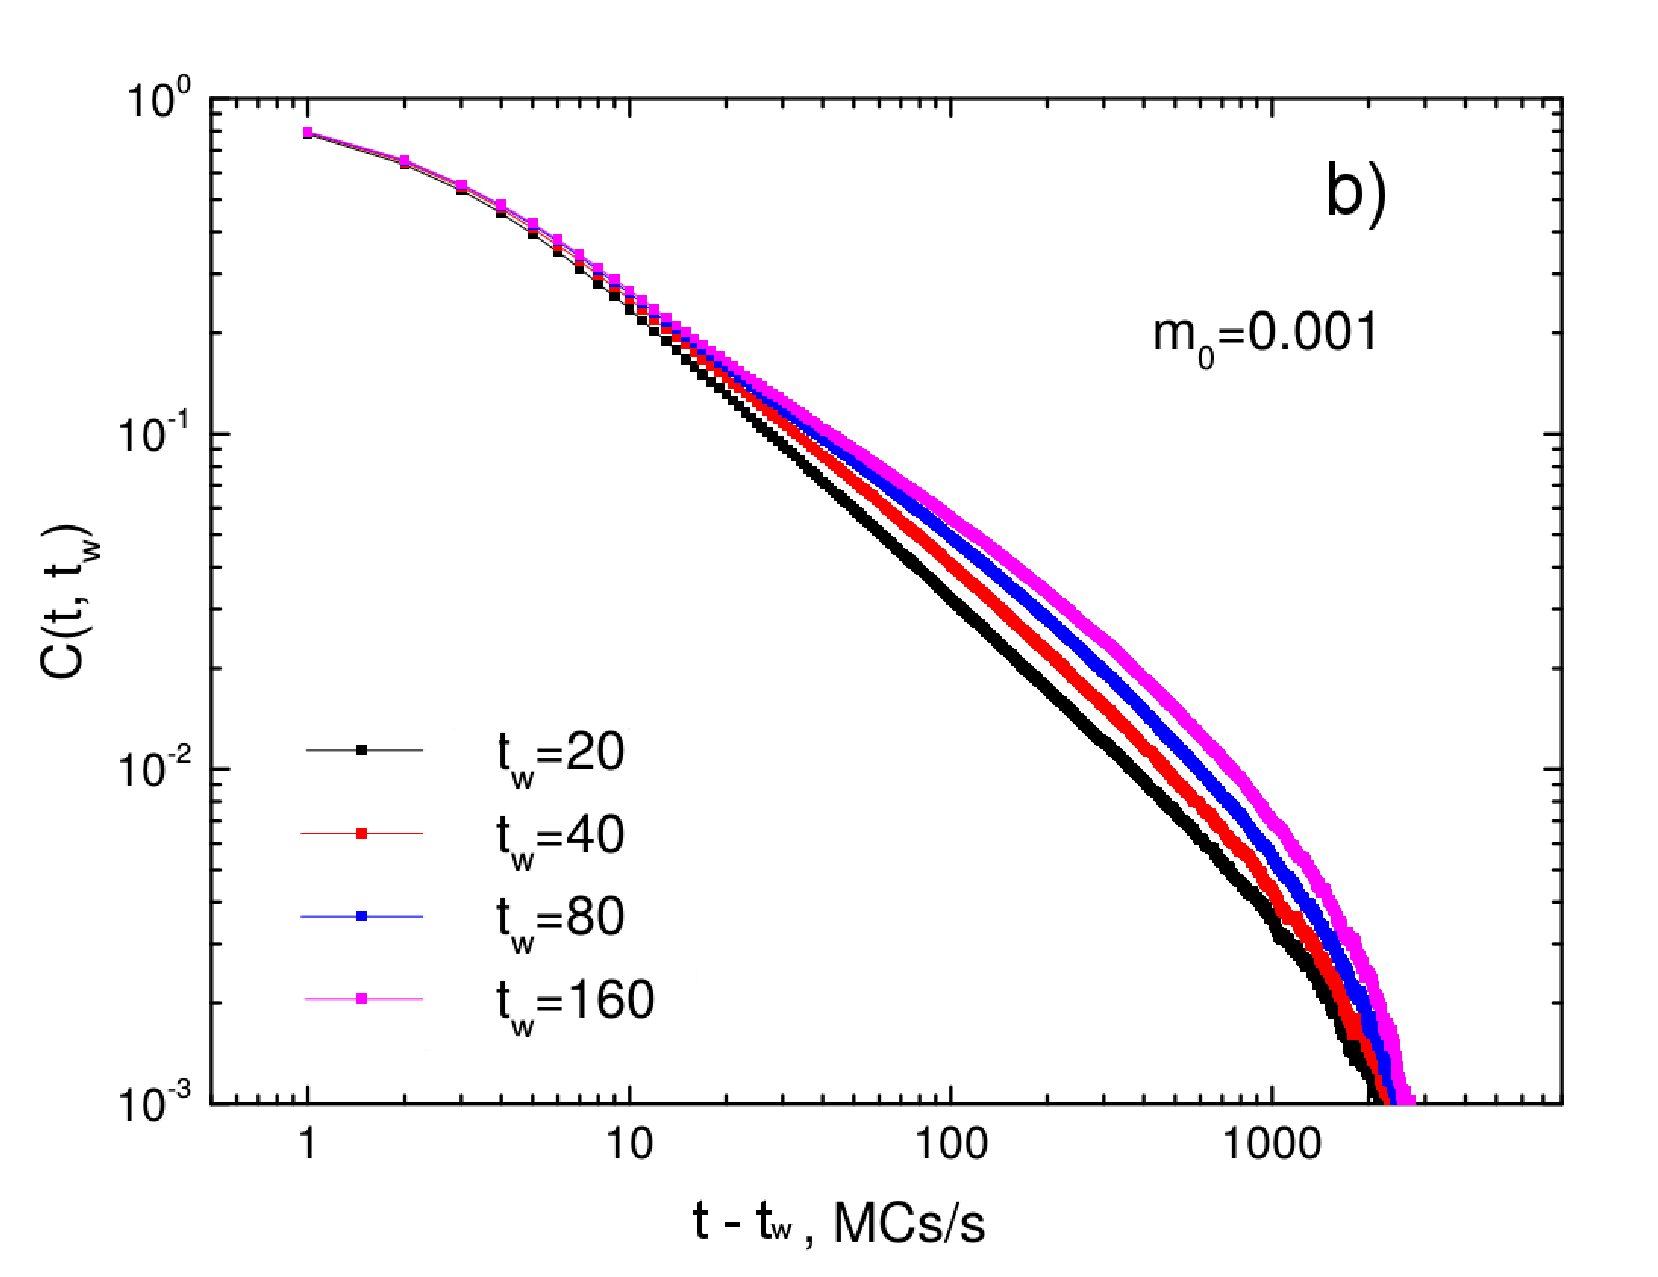
\includegraphics[width=6.77cm]{corr_ageing_0001}
\end{minipage}

\caption{\label{fig:m1_all} Time dependence of the autocorrelation
function $C(t, t_w)$ for various waiting times $t_w$ with evolution
from \textbf{a)} the completely initial state with $m_0 = 1$ and
\textbf{b)} the low-temperature initial state with $m_0 = 0.001$.}

\end{center}
\end{figure}

В таблице \ref{tab:m1_scail} приведены значения критических показателей с учетом попрвки к скейлингу, полученные при моделировании системы из начального низкотемпературного состояния с $m_o = 1$.

\begin{table}
\caption{Значения индексов, полученных при учёте ведущих поправок к скейлингу. $m_0 = 1$. \label{tab:m1_scail}}
\begin{center}
\begin{tabular}{c|c|c}
  Индекс             & $p = 0.5$ & $p = 0.6$  \\ \hline
  {$\beta$} & {$0.314(51)$} & {$0.354(61)$} \\
  {$\nu$} & {$0.711(50)$} & {$0.710(55)$} \\
  {$z$} & {$2.655(42)$} & {$2.559(48)$} \\
  {$\beta/\nu$}  & {$0.442(25)$} & 0.490(24) \\
  \hline
  {$(\omega/z)_{av}$}  & \multicolumn{2}{c}{$0.103(11)$}
\end{tabular}
\end{center}
\end{table}

\begin{table}
\caption{Значения индексов, полученных при учёте ведущих поправок к скейлингу при моделировании из начального состояния с $m_0 \ll 1$. }
\label{tab:m0_scail}
\begin{center}
\begin{tabular}{c|c|c}
  Индекс             & $p = 0.5$ & $p = 0.6$  \\ \hline
  {$\theta'$} & {$0.192(26)$} & {$0.194(41)$} \\
  {$z$} & {$2.740(90)$} & {$2.760(110)$} \\
  {$z(F_2)$} & {$2.647(63)$} & {$2.627(59)$} \\
  {$\beta/\nu$}  & {$0.430(60)$} & 0.479(81) \\
  \hline
  {$(\omega/z)_{av}$}  & \multicolumn{2}{c}{$0.149(30)$}
\end{tabular}
\end{center}
\end{table}

\section{Анализ результатов и выводы}
В данной работе было проведено численное исследование сильнонеупорядоченной модели Изинга для концентраций спинов $p = 0.5$ и  $p = 0.6$. Определены значения критических индексов $\theta'$, $\beta$, $\nu$, $z$ и $\omega$ с учетом ведущей поправки к скейлингу.


Численные исследования были проведены с привлечением ресурсов СКИФ МГУ "Чебышев".


\begin{thebibliography}{99}

\bibitem{lit:Harris}
A.~B.~Harris, J. Phys. C \textbf{7}, 1671 (1974).

\bibitem{lit:HalperinHoenberg}
P.~C.~Hohenberg and B.~I.~Halperin, Rev. Mod. Phys. \textbf{49}, 435 (1977).

\bibitem{lit:Folk}
Фольк Р., Головач Ю., Яворский Т. УФН, Т. 173. № 2. (2003).

\bibitem{lit:Janssen}
H.~K.~Janssen, B.~Schaub, and B.~Schmittmann, Z. Phys. B \textbf{73}, 539 (1989).

\bibitem{lit:Huse}
D. A. Huse, Phys. Rev. B, \textbf{40} 304 (1989).

\bibitem{lit:Zheng}
B. Zheng, Int. J. Mod. Phys. B, \textbf{12} 1419 (1998).

\bibitem{lit:Jaster}
A. Jaster, J. Mainville, L. Sch\"eulke, and B. Zheng, J. Phys.
A \textbf{32} 1395 (1999).

\bibitem{lit:Luo}
H. J. Luo, L. Sch\"eulke, and B. Zheng, Phys. Rev. E, \textbf{64} 036123 (2001).

\bibitem{lit:Schehr}
Schehr G., Paul R., J. Phys: Conf. Series. \textbf{40} 27 (2006).

\bibitem{lit:Hasenbusch}
M. Hasenbusch, A. Pelissetto, and E. Vicari, J. Stat. Mech.: Theory Exp., P11009 (2007).

\bibitem{lit:Rosov88}
Rosov N., Eibsch\"utz M., Hohenemser C., Kleinhammes A., Lidbjork P., Phys. Rev. B., \textbf{37}, (1988).

\bibitem{lit:Prudnikov_FT}
Прудников В.В., Прудников П.В., Криницин А.С., ТМФ. \textbf(147) 137 (2006).

\bibitem{lit:Alves}
Alves N.A., Da Silva R., Drugowich de Felicio J.R., Phys. Lett. A. \textbf{298} 325 (2002).

\bibitem{lit:Tc}
Прудников В.В., Прудников П.В. Вакилов А.Н., Криницын А.С., ЖЭТФ. Т. 132. № 2. С. 417 (2007).

\bibitem{lit:Wegner}
Wegner F.J., Phys. Rev. B. \textbf{5} 4529 (1972).

\bibitem{lit:Prudnikov_PRE2010}
V.~V.~Prudnikov, P.~V.~Prudnikov, A.~S.~Krinitsyn, A.~N.~Vakilov,
E.~A.~Pospelov, and M.~V.~Rychkov, Phys. Rev. E \textbf{81}, 011130 (2010).

\bibitem{lit:Pesissetto}
A. Pelissetto, E. Vicari, Phys. Rev. B, \textbf{62}, 6393 (2000).

\bibitem{lit:Rosov92}
Rosov N., Eibsch\"utz M., Hohenemser C., Phys. Rev. B., \textbf{46} 3452 (1992).

\bibitem{lit:Parisi}
Parisi G., Ricci-Tersenghi F., Ruiz-Lorenzo J.J., Phys. Rev. E., \textbf(60) 5198 (1999).

\bibitem{lit:Murtazaev}
Муртазаев А. К., УФН, Т. 176. № 10. С. 1119 (2006)

\bibitem{lit:Heuer}
Heuer H.-O., J. Phys. A. \textbf{26} 333 (1993).

\end{thebibliography}

\end{document}
